Im Jahr 2009 veröffentlichte Ryan Dahl das Framework Node.js, das auf Googles V8-Engine, welche auch als JavaScript-Engine in Googles Browser Chrome zum Einsatz kommt, basiert und sich hervorragend für hochperformante, skalierbare und schnelle Webanwendungen eignet. Zudem ermöglicht es Webentwicklern die Entwicklung von serverseitigem JavaScript-Code. \-[NodeJS 1.0]


\textbf{- Architektur TODO Aufzählung}
Eine wesentliche Eigenschaft von Node.js ist die hohe Performance. Im Folgenden soll der Unterschied der Node.js-Architektur zu traditionellen Webservern und der damit verbundenen höheren Performance dargestellt werden.
\newline

Herkömmliche Webserver erstellten zunächst für jede ankommende Anfrage einen neuen Thread. Dieses Vorgehen ist eng mit steigendem Speicher- und Rechenaufwand verbunden. Um sich Rechenzeit, die durch die Erstellung und Zerstörung von Threads entstanden, zu sparen, wurden Threadpools eingerichtet. Dieser Threadpool enthält mehrere Threads, denen Aufgaben zugewiesen werden können. Nach erfolgreicher Abarbeitung einer Operation kann einem Thread eine weitere Aufgabe zugeordnet werden.
\newline

Es bleibt aber ein weiteres Problem: Bei der Anfragenabarbeitung kann es zu einer Form von blockierender Ein- und Ausgabe (Blocking Input/Output kurz Blocking I/O) kommen: zum Beispiel beim Suchen in einer Datenbank oder dem Laden einer Datei im Dateisystem. Während der Abarbeitung wartet der Thread solange, bis die Operation ein Ergebnis zurückwirft und belegt dabei weiterhin Speicherplatz. Bei hohem Anfragen-aufkommen kommt es dadurch zu einer hohen Speicherauslastung des Servers. Zudem kosten die Kontextwechsel zwischen den Threads im Betriebssystem weitere Rechenzeit. [Node.js 1.05] Man spricht bei diesem Architekturkonzept auch vom Multi-Threaded Server.
\newline

\begin{figure}[h]
\centering
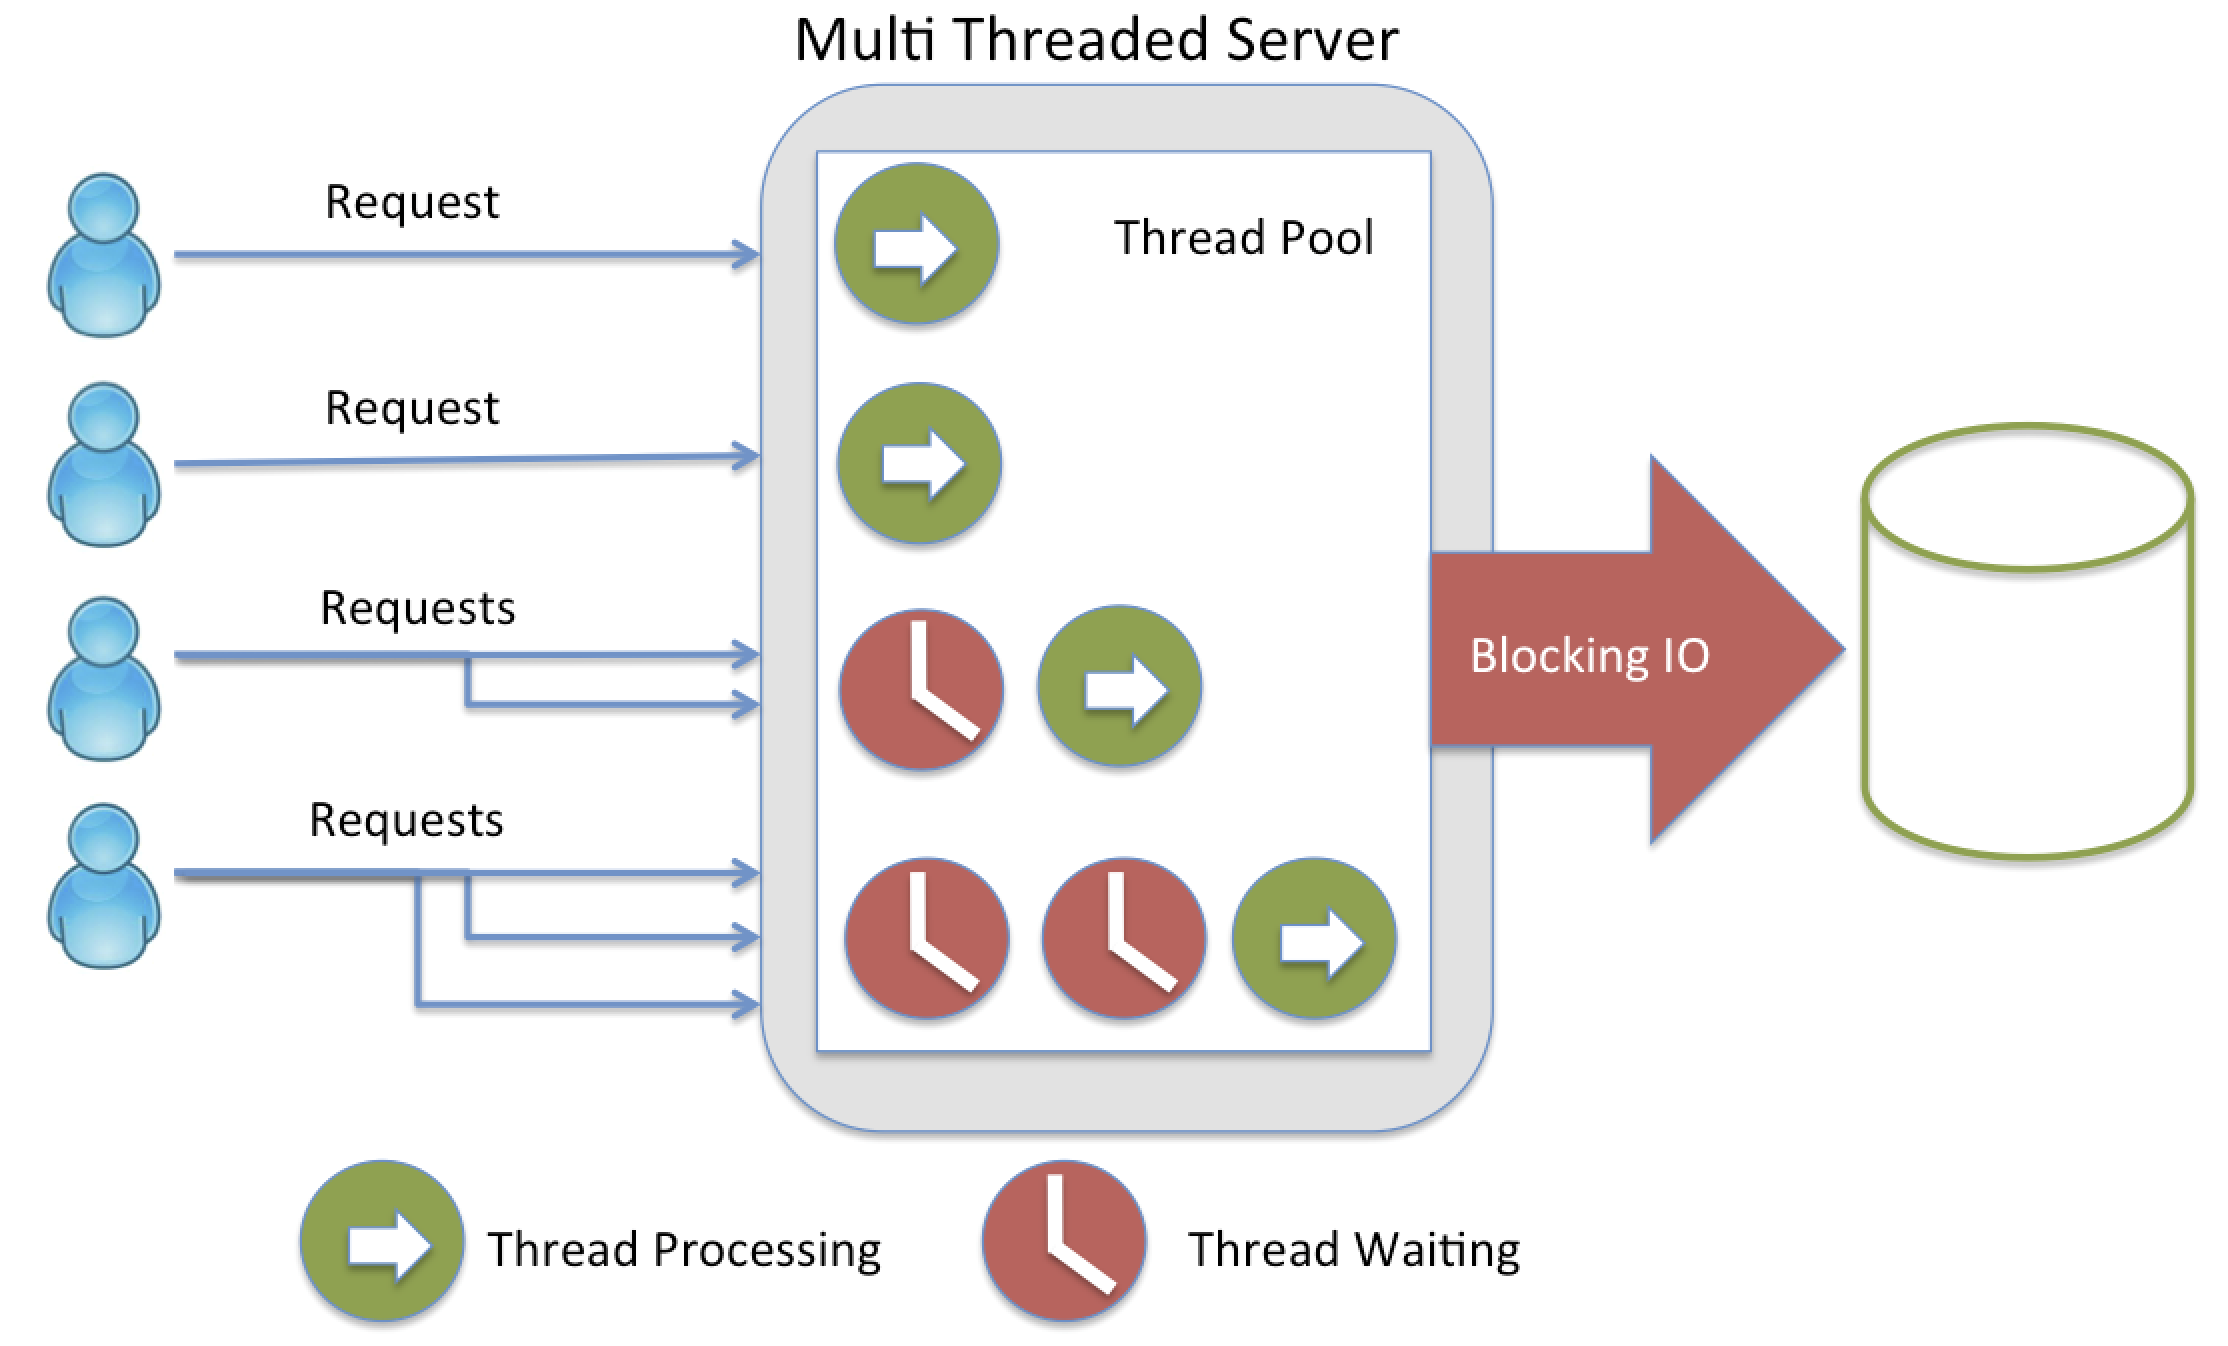
\includegraphics[width=10cm, height = 5.5cm]{images/nodejs_otherthreading.png}
\caption{Multithreaded / Blocking I/O [Nodejs 1.1]}
\end{figure}
 
\newpage

Node.js verfolgt einen anderen Ansatz: Anfragen werden nur in einem einzigen Thread, dem Hauptthread, abgearbeitet und in einer Warteschlange verwaltet. Dadurch bleiben Kontextwechsel zwischen Threads erspart. Hierbei handelt es sich also um einen Single-Threaded Server. Der Hauptthread verwaltet eine Schleife, die sogenannte Event Loop, die permanent Anfragen aus der Event-Warteschlange überprüft und Ereignisse, die von Ein- und Ausgangsoperationen ausgerufen werden, verarbeitet.
\newline

Bei Ankommen einer Nutzeranfrage an einen Node.js Server wird zunächst in der Event Loop geprüft, ob diese Anfrage Blocking I/O benötigt. Falls nicht, kann die Anfrage direkt bearbeitet werden und die Antwort an den Nutzer zurückgesendet werden. 
\newline

Im anderen Fall wird einer von Node.js interner Workern, welche prinzipiell auch Threads sind, aufgerufen, um die jeweilige Operation auszuführen. Dabei wird eine Callback-Funktion mitgegeben, die vom Worker aufgerufen wird, sobald die Operation ausgeführt wurde. Diese Callback-Funktion ist kann anschließend als Ereignis von der Event Loop registriert werden. Man spricht hierbei auch von ereignisgesteuerter Architektur. [1.4]
\newline
 
\begin{figure}[h]
\centering
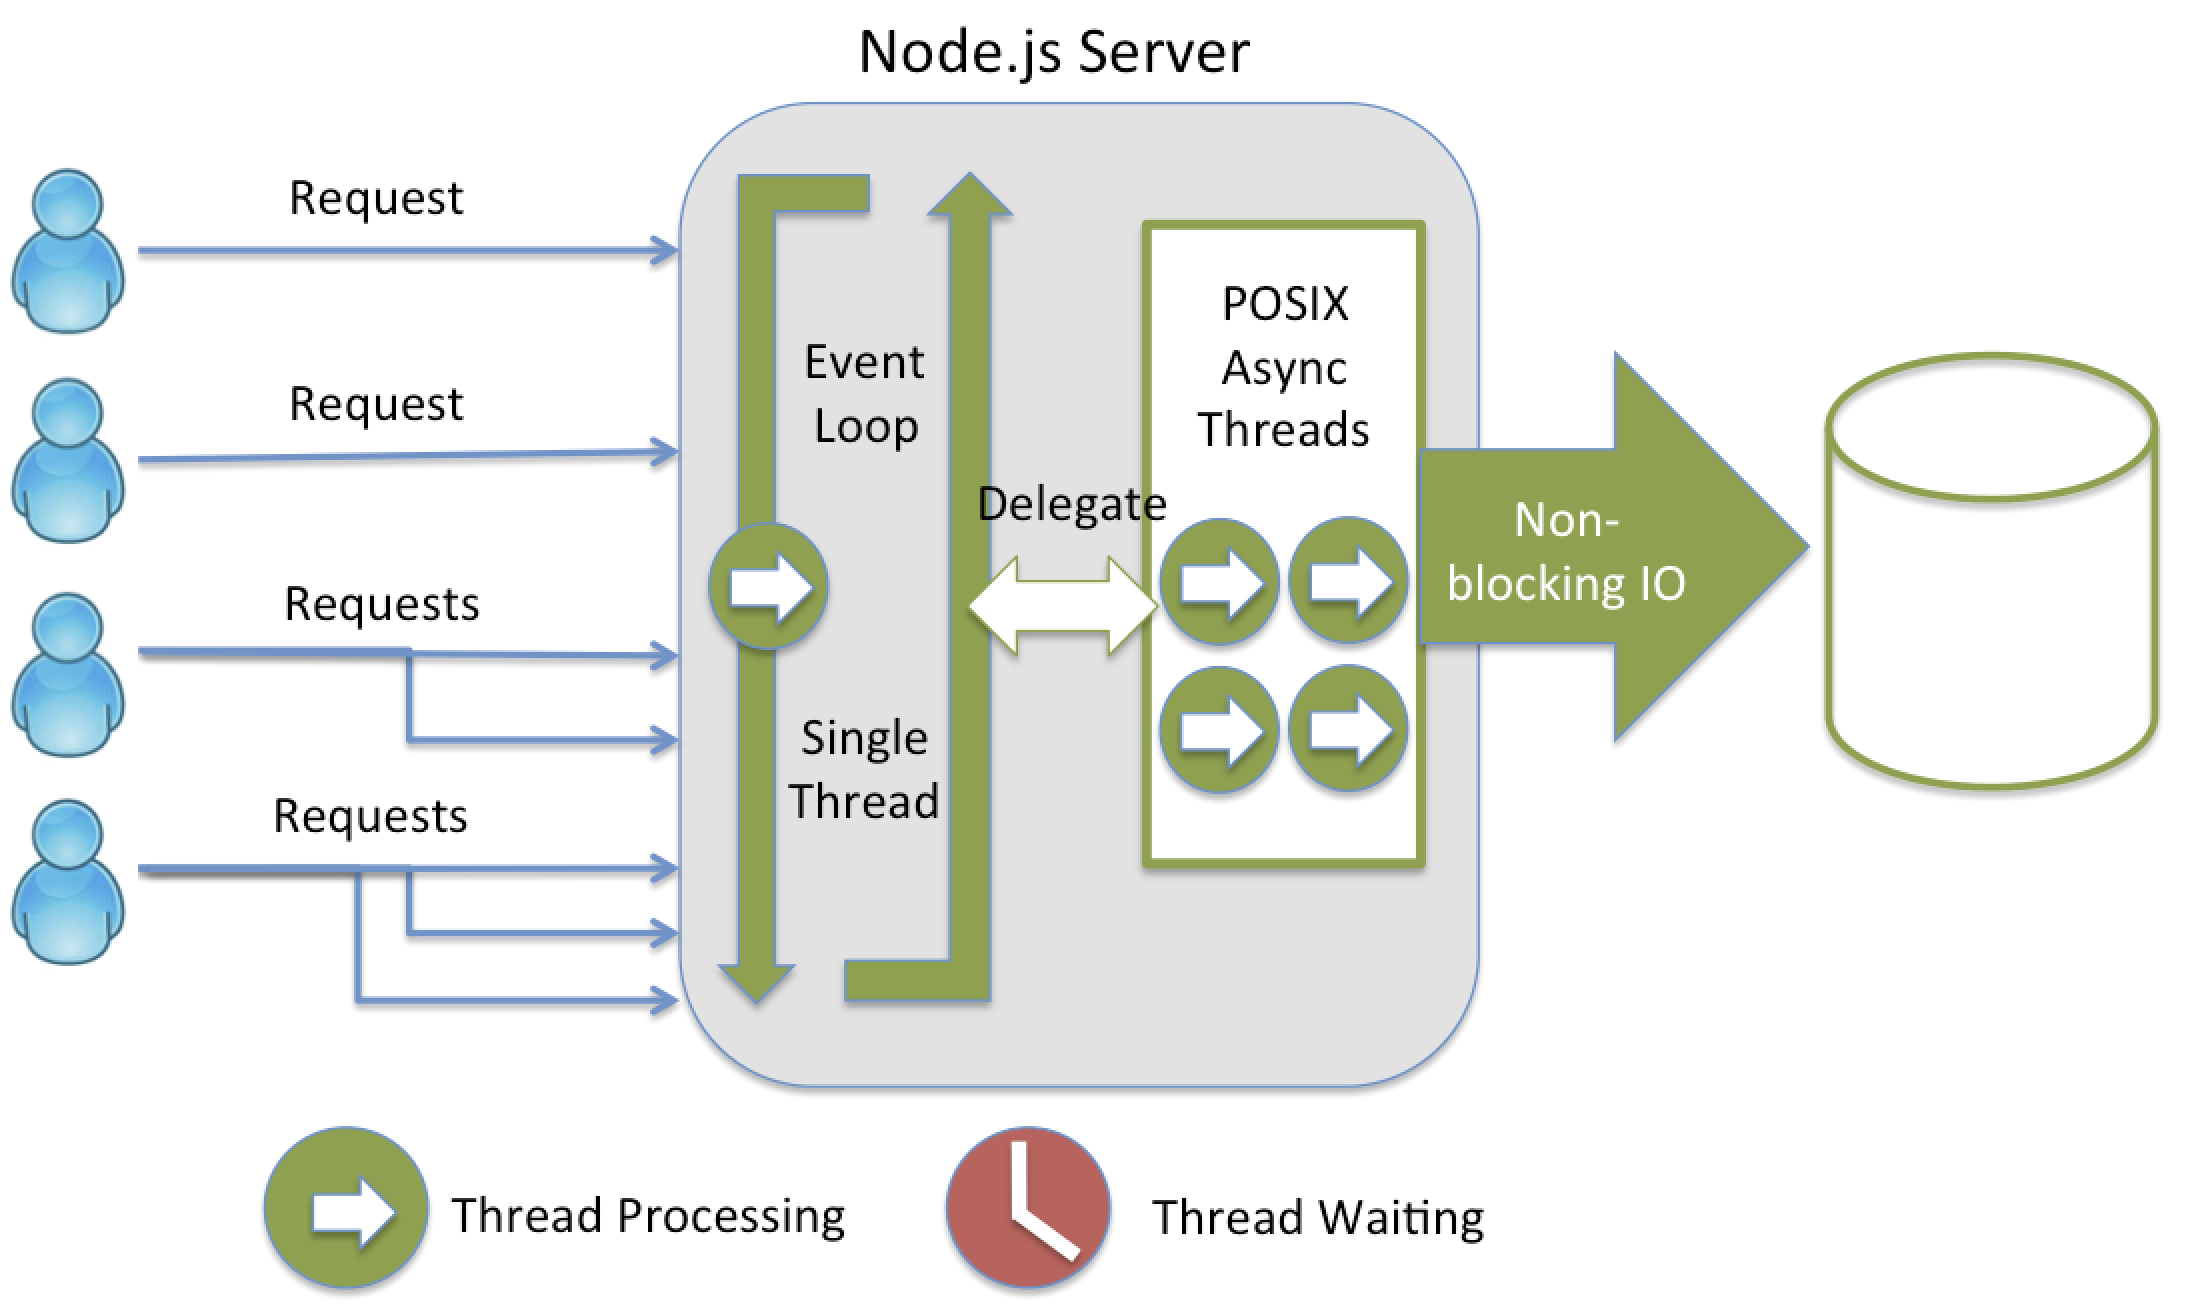
\includegraphics[width=10cm, height = 5.5cm]{images/nodejs_nodethreading.png}
\caption{ Single Threaded / Non Blocking I/0 [Nodejs 1.1]}
\end{figure}
 
 
Der große Vorteil hierbei ist, dass der Hauptthread trotz der blockierenden Ein- und Aus\-gabeoperationen nicht anhält, und weitere Anfragen bearbeiten kann. (Non Blocking I/O - Prinzip) 
\newline

\newpage
\textbf{- Module TODO Aufzählung}

Module stellen in Node.js Software-Komponenten dar, die Objekte und Funktionen nach außen hin bereitstellen sollen. Sie können aus einer Skriptdatei oder einem Verzeichnis von Dateien bestehen. Module können als einzelne Default-Komponente, die den Hauptteil des Moduls repräsentiert, exportiert werden. Bei der anderen Möglichkeit, des sogenannten ‚benannten Exports‘ werden die zu exportierenden Komponenten dagegen explizit angegeben. Letzteres ist in nachfolgender Abbildung dargestellt. 
\newline
  
\begin{figure}[h]
\centering
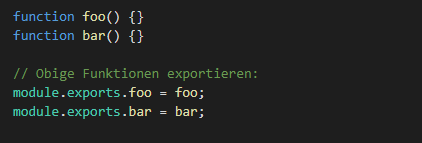
\includegraphics{images/nodejs_moduleExport.PNG}
\caption{Benannter Export von Modulen}
\end{figure}
 
Für den Import stehen verschiedene Möglichkeiten zur Verfügung. Im folgender Abbildung ist ein Import über die require()-Funktion dargestellt. Mit mitgeliefertem Modul-Pfad als Parameter gibt diese Funktion ein Objekt des Moduls wieder, dass die exportierten Objekte (und Funktionen) enthält.
\newline
  
\begin{figure}[h]
\centering
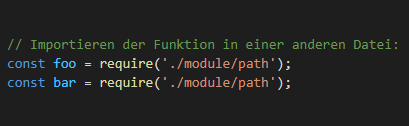
\includegraphics{images/nodejs_moduleImport.PNG}
\caption{Import von Modulen}
\end{figure}

Caching TODO
Modules are cached after the first time they are loaded. This means (among other things) that every call to require('foo') will get exactly the same object returned, if it would resolve to the same file.\newline
Provided require.cache is not modified, multiple calls to require('foo') will not cause the module code to be executed multiple times. This is an important feature. With it, "partially done" objects can be returned, thus allowing transitive dependencies to be loaded even when they would cause cycles. [nodejs 1.21]


\textbf{- npm TODO Aufzählung}
Ehemals als Node Package Manager bekannt, ist npm ein Paketmanager für Node.js, entwickelt 2010 von Isaac Z. Schlueter [nodejs 1.3] Es verwaltet ein öffentliches Repository (ein digitales Software-Verzeichnis im Internet) unter dem Name npm Registry. In dem Verzeichnis werden weit über 1 Millionen Pakete (Module) angeboten. [1.4] Der Großteil kann unter freier Lizenz verwendet werden. Mit npm können Module installiert, aktualisiert, entfernt und gesucht werden. Node.js liefert seit seiner Version 0.6.3 npm standardmäßig bei der Installation mit. [1.5]

\textbf{Express TODO Aufzählung}
„Express ist ein einfaches und flexibles Node.js-Framework von Webanwendungen, das zahlreiche leistungsfähige Features und Funktionen für Webanwendungen und mobile Anwendungen bereitstellt.“ [nodejs 1.6] Es wurde im November 2010 von Douglas Christopher Wilson und weiteren Entwicklern veröffentlicht und erweitert Node.js um das Abarbeiten verschiedener HTTP-Methoden, das separate Abarbeiten von Anfragen mit verschiedenen URL-Pfaden sowie weiterer nützlicher Möglichkeiten. Im Grunde handelt es sich bei Express um ein Modul, dass durch den npm Package Manager heruntergeladen werden kann. Die aktuelle Version zum Zeitpunkt der Dokumentation [??] ist 4.17.1. [nodejs 1.65] \newline
\newline
\textbf{Beispiel}
 \newline

Das Erstellen einer einfachen Express-Applikation wird im folgenden Beispiel dargestellt:\newline

\begin{figure}[h]
\centering
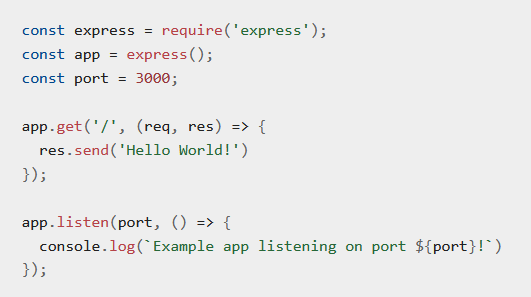
\includegraphics{images/nodejs_express_einfacherWebserver.PNG}
\caption{Einfacher Webserver [nodejs 1.8]}
\end{figure}


Die require()-Funktion importiert das Express-Modul und gibt ein Express-Objekt zurück. Dieses Objekt als Funktion aufgerufen gibt wiederum ein Objekt der Express-Applikation zurück, welche traditionell „app“ genannt wird, das Kernstück des Express-Frameworks ist und sämtliche Methoden wie das Weiterleiten von HTTP Anfragen, das Konfigurieren von Middleware oder das Modifizieren des app-Verhaltens beinhaltet. [nodejs 1.8]\newline 

Im mittleren Block befindet sich eine Routendefinition. Die app.get() Funktion spezifiziert eine Callback-Funktion, die ein „request“- und „response“-Objekt als Parameter erhält und aufgerufen wird, sobald eine HTTP Anfrage der Methode GET mit dem Pfad ‚/‘ empfangen wird. Das Request-Objekt enthält sämtliche Informationen über die HTTP-Anfrage. Das Response-Objekt kann dagegen in der Callback-Funktion mit Informationen gefüllt werden und über die send()-Funktion als HTTP-Antwort an den Sender zurückgesendet werden.\newline

Der unterste Block startet den Webserver auf dem mitgegebenen Port über die Funktion app.listen(). Ihr kann auch eine Callback-Funktion mitgegeben werden, die aufgerufen wird, sobald der Server erfolgreich gestartet ist.\newpage

\textbf{Middleware}
\newline
Express arbeitet nach dem Middleware-Konzept. Darunter versteht man Funktionen, die für die Verarbeitung von Anfragen hintereinandergeschaltet werden können. Jede Middleware hat Zugriff auf das Anfrageobjekt, das Antwortobjekt und die jeweils nächste Middleware-Funktion. [nodejs 1.9]
Dabei kann die HTTP-Request direkt terminiert oder an die nächste Middleware gesendet werden. Die Verkettung der Middleware-Funktionen wird in folgender Abbildung illustriert: \newline

\begin{figure}[h]
\centering
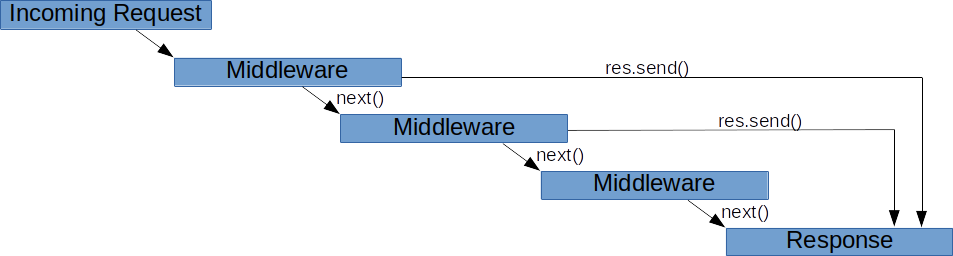
\includegraphics[width=12cm]{images/nodejs_middleware.png}
\caption{Middleware [nodejs 2.0]}
\end{figure}

\textbf{Middleware: express.json}
\newline

Hierbei handelt es sich um eine in express eingebaute Middleware, die die in JSON formatierten Daten im Nachrichtenrumpf aus einer eingehenden HTTP-Anfrage grammatisch analysiert.  Dabei ist zu beachten, dass der Nachrichtenrumpf nur dann analysiert wird, wenn bei der Anfrage eine Header-Informationen namens „Content-Type“ mit dem entsprechenden JSON-Typ als Wert übergeben wird. Nach erfolgreicher Analyse erstellt die Middleware aus den JSON-Informationen eine neues body-Objekt innerhalb des übergebenen request-Objekts. [nodejs 2.1]
\newline

\begin{figure}[h]
\centering
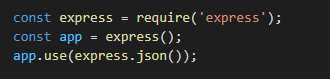
\includegraphics{images/nodejs_expressJson.PNG}
\caption{Express.json Middleware benutzen}
\end{figure}

\newpage
\textbf{Middleware: Router}
\newline

Unter dem Begriff Routing (Weiterleitung) versteht man im Kontext von Express „[...] die Definition von Anwendungsendpunkten (URIs) und deren Antworten auf Clientanforderungen.“ [nodejs 2.15]
\newline

Die in express eingebaute Middleware express.Router ermöglicht es, modular einbindbare Routenhandler (Weiterleitungsroutinen) zu erstellen. Eine Router-Instanz ist als vollständiges Middleware- und Routingsystem zu sehen und wird deshalb auch als „Mini-App“ angesehen. Der sich durch die Modularität herausziehende Vorteil ist, dass folglich unterschiedliche Anwendungsendpunkte auf entsprechende Dateien ausgelagert werden können.
\newline

\begin{figure}[h]
\centering
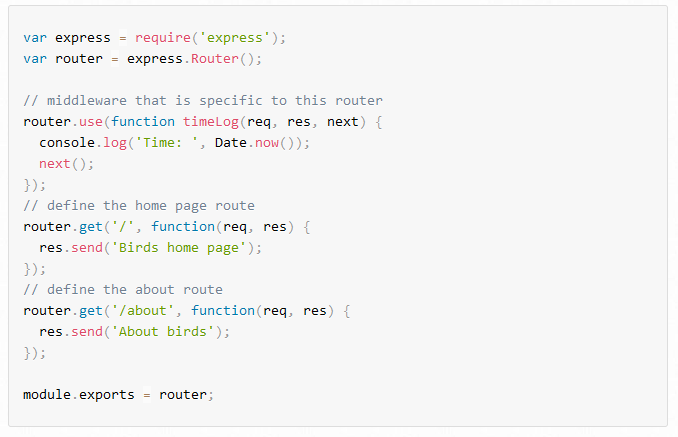
\includegraphics[width=14cm]{images/nodejs_expressRoutererstellen.PNG}
\caption{Routinghandler erstellen[nodejs 2.2]}
\end{figure}

In oberem Beispiel wird ein Routerhandler für das Verzeichnis ‚/birds‘ mit eigen implementierter Middleware und zwei Anwendungsendpunkte ‚/‘ (bezieht sich auf das Stammverzeichnis) und ‚/about‘ erstellt. Der Code wird unter der Datei birds.js abgespeichert. 
Abschließend kann das Routermodul in die Anwendung geladen werden: 
\newline

\begin{figure}[h]
\centering
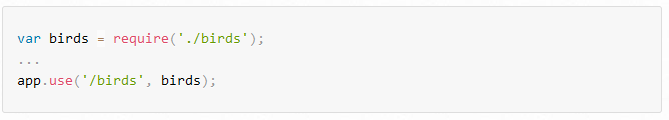
\includegraphics[width=14cm]{images/nodejs_expressRouterbenutzen.PNG}
\caption{Routinghandler benutzen[nodejs 2.2]}
\end{figure}

\newpage
\textbf{- Mongoose TODO Aufzählung}
Mongoose ist ein öffentliches Modul, dass zum Zeitpunkt der Dokumentation[??] im npm Package Manager in der Version 5.12.3 zur Verfügung steht. [nodejs 2.4] Bei diesem Modul handelt es sich um ein Object-Document Mapper (ODM), der es ermöglicht, asynchron mit einer NoSql-Datenbank zu kommunizieren. Mongoose ist der populärste und am weitest von MongoDB unterstützte ODM. [nodejs 2.55] Es unterstützt neben transparenter Persistenz auch die Datenvalidierung, das Erstellen von Abfragen (Queries), das Schreiben von logischem Business Code und die Übertragung zwischen Objektem im Code und der Repräsentierung dieser Objekte in der Datenbank.
\newline

\textbf{Object Document Mapping (ODM)}
\newline
Object-Relational Mappers (ORM) finden hauptsächlich Einsatz in objektorientieren Anwendungen, dessen Daten in relationalen Datenbanken sind. Dabei werden die Tabellen in persistente Objekte gemappt.
Das Mappen ist aber auch für NoSQL-Datenbanken nützlich. [nodejs 2.56] Die meistverbreiteten NoSQL-Datenbanken basieren auf Dokument-Systemen. Dementsprechend werden für diese Datenbanken Object-Document Mapper für das Mappen zwischen Dokumenten und Objekten genutzt. Einige ODM’s sind Mongoose[nodejs 2.7], Morphia [nodejs 2.8], Doctrine[nodejs 2.9] und Mandango[nodejs 3.0].
NoSQL Mapper nutzen vom Entwickler definierte Datenschemata, die das Objekt beschreiben. Ein daraus abgeleitetes Model-Objekt ermöglicht dann die Kommunikation zwischen dem im Schema beschriebenen Objekt und der entsprechenden Datenbank-Collection.
\newline

\textbf{Schema}
\newline
Mongoose-Schemata definieren die Struktur der gespeicherten Daten einer MongoDB-Collection in der Anwendungsschicht und werden in der JSON-Notation beschrieben. Dokumentenbasierte Datenbanken wie MongoDB enthalten für jede Wurzelentität [??] eine Collection. Mongoose Schemata werden für jede Collection und jede Nichtwurzel-entität[??] definiert. Innerhalb der JSON-notierten Schemabeschreibung können den einzelnen Eigenschaften bestimmtes Verhalten zugeordnet werden. Zum Beispiel lässt sich explizit der Datentyp angeben (type), eine Eigenschaft verpflichtend (required) oder in Kleinbuchstaben einstellen (lowercase).
\newline

\begin{figure}[h]
\centering
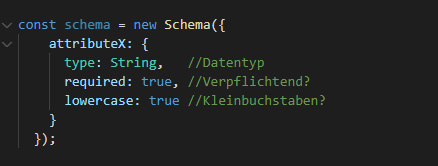
\includegraphics{images/nodeJS_mongooseSchema.PNG}
\caption{Mongoose Schema - Beispiel}
\end{figure}

\newpage
\textbf{Model}
\newline
Ein Model in Mongoose ist ein aus einer Schemadefinition erstellter Konstruktor, aus denen Objekte instanziiert werden können. Diese Instanzen werden auch ‚documents‘ genannt. Sie stehen in direkter Verbindung zu den jeweiligen Collections der verbundenen Datenbank und enthalten Methoden für die persistente Speicherung, Bearbeitung oder Löschung. Beispielsweise wird beim Abspeichern einer Mongoose Instanz eines Models die entsprechende Collection in der Datenbank erzeugt, sofern sie noch nicht vorhanden ist. Eine Konvention in Mongoose sieht vor, dass der Name eines Models dem Singular eines Nomens entspricht, während die Collections nach dem Plural dieses Namens beschrieben werden. [nodejs 3.2] Im folgenden Beispiel wird ein Model über die mongoose.model()-Funktion erstellt unter Angabe des Modelnamens und dem zu verwendenden Schema. Dieses Model wird über module.exports nach außen zur Verfügung gestellt.

\begin{figure}[h]
\centering
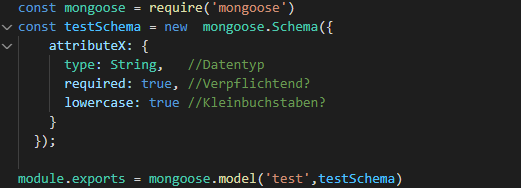
\includegraphics{images/nodeJS_mongooseModell.PNG}
\caption{Model erstellen und exportieren}
\end{figure}

An anderer Stelle kann das Model nun importiert werden. Aus dem Model kann ein Objekt instanziiert werden, welches über die save()-Funktion in der Datenbank gespeichert werden kann.

\begin{figure}[h]
\centering
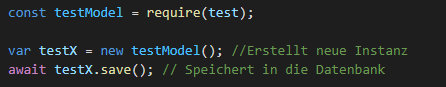
\includegraphics{images/nodeJS_mongooseModellimport.PNG}
\caption{Model importieren, Objekt instanziieren und persistent speichern}
\end{figure}

Mongoose Models enthalten ohne Instanziierung des Weiteren auch Schnittstellen, um Daten der zugehörigen Collection zu kreieren, abfragen, bearbeiten oder löschen. (Create, Receive, Update, Delete oder auch kurz CRUD).
\newline
\newpage
\begin{figure}[h]
\centering
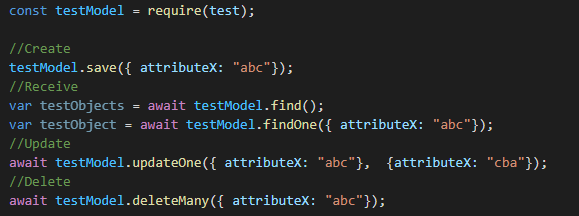
\includegraphics{images/nodeJS_mongooseModellCRUD.PNG}
\caption{CRUD-Besipielfunktionen eines Mongoose-Models}
\end{figure}

\textbf{Verbindung}
\newline
Verbindung zur Datenbank kann über die connect()-Funktion mit Angabe der genutzten Datenbank und des Datenbankpfads. Über das mongoose.connection-Objekt können auf Verbindungsereignisse reagiert werden. 
\newline


\begin{figure}[h]
\centering
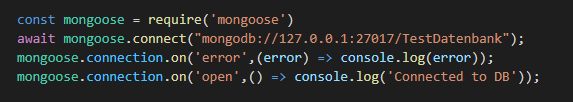
\includegraphics{images/nodeJS_mongooseVerbindung.PNG}
\caption{Mongoose: Verbindung zur Datenbank aufbauen}
\end{figure}

Für den Verbindungsaufbau können weitere Option übergeben werden. Dafür kann ein Objekt wie in folgendem Beispiel erstellt werden, dass die zugehörigen Optionen als Attribute beinhaltet. 
\newline


\begin{figure}[h]
\centering
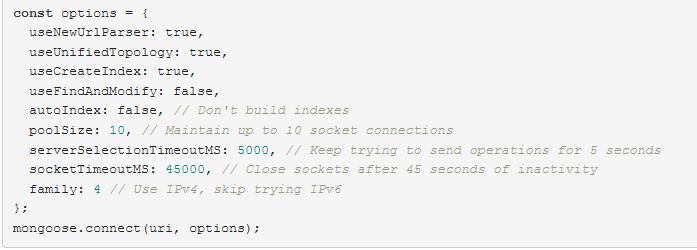
\includegraphics[height=5.5cm]{images/nodeJS_mongooseVerbindungOptions.PNG}
\caption{Mongoose Verbindungsoptionen[nodejs 3.3] }
\end{figure}

\newpage
\textbf{- Weitere Module TODO Aufzählung}
TODO warum Tabelle oben?

\begin{table}[]
\begin{center}
    \begin{tabular}{| l | p{8cm} |}
    \hline
    Express-Modul & Beschreibung \\ \hline
    fs & Erlaubt die Interaktion mit dem Dateisystem.\newline
	Zum Beispiel Schreiben/Lesen von Dateien.\\
    
    \hline
    http & Ermöglicht Datentransfer über das Protokol HTTP und das Abhören eines Ports.  \\
    
    \hline
	https & Gesicherte Variante zu HTTP mit SSL.\newline
	Benötigt Private Key und Zertifikat.  \\
	
    \hline    
    firebase-admin & Ermöglicht die Verbindung zu Google Firebase 			Cloud. \\ 
    
    \hline    
    node-cron & Ermöglicht das Einstellen von sich wiederholenden 			Aufgaben zu bestimmten Zeitintervallen.  \\
    \hline
    \end{tabular}
\end{center}
\caption{Module}
\end{table}
